%==============================================================================
% Sjabloon poster bachproef
%==============================================================================
% Gebaseerd op document class `a0poster' door Gerlinde Kettl en Matthias Weiser
% Aangepast voor gebruik aan HOGENT door Jens Buysse en Bert Van Vreckem

\documentclass[a0,portrait]{hogent-poster}

% Info over de opleiding
\course{Bachelorproef}
\studyprogramme{toegepaste informatica}
\academicyear{2023-2024}
\institution{Hogeschool Gent, Valentin Vaerwyckweg 1, 9000 Gent}

% Info over de bachelorproef
\title{Machine learning-technologie toepassen om relevante masterdata uit bedrijfsdocumenten te halen}
%\subtitle{Ondertitel (eventueel)}
\author{Jamie Van Schuerbeek}
\email{jamie.vanschuerbeek@student.hogent.be}
\supervisor{Chloé De Leenheer}
\cosupervisor{Alexander Jacobs (Alluvion)}

% Indien ingevuld, wordt deze informatie toegevoegd aan het einde van de
% abstract. Zet in commentaar als je dit niet wilt.
\specialisation{Functional \& Business Analysis}
\keywords{SAP, Master Data Management, Document Information Extraction}
\projectrepo{https://github.com/jamievschuerbeek/proof-of-concept-bachelorproef}

\begin{document}

\maketitle

\begin{abstract}
  In het dynamische landschap van de moderne bedrijfsvoering, is het efficiënt master data uit omvangrijke bedrijfsdocumenten halen cruciaal. In de meeste bedrijven wordt dit nog steeds beschouwd als een overbodige handmatige activiteit. Masterdata, de kerninformatie die de belangrijkste entiteiten van een organisatie definieert zoals klanten, producten en leveranciers, speelt een belangrijke rol bij geïnformeerde besluitvorming en strategische planning. Hoe kan machine learning-technologie worden toegepast om relevante masterdata uit bedrijfsdocumenten te halen? Met dit onderzoek zou Alluvion graag een antwoord op deze vraag willen krijgen door de verschillende manieren om dit proces te automatiseren te ontdekken.
  
  Om dit doel te bereiken begint deze studie met een onderzoek naar deep learning technieken zoals die kunnen gebruikt worden om dit doel te bereiken. Vervolgens wordt er ook onderzoek gedaan naar bestaande tools die deze technieken implementeren. Deze tools worden vervolgens geëvalueerd op basis van verschillende factoren zoals prijs, kwaliteit, integratie met SAP platformen en gebruiksvriendelijkheid om zo een tool te kunnen bepalen waarmee een proof of concept wordt gemaakt.
  
  Een praktische implementatie in de vorm van een proof of concept toont aan hoe de SAP BER service gebruikt kan worden om een praktische toepassing te maken die masterdata uit bedrijfsdocumenten kan halen. Dit proof of concept dient als een basis voor verdere ontwikkeling van een product dat Alluvion kan gebruiken om verdere verbeteringen aan te maken om op die manier een volledig product te bekomen. SAP BER samen gepaard met SAP Fiori vormt een eenvoudige manier om applicaties te bouwen die kunnen helpen bij het automatiseren van masterdata extractie uit bedrijfsdocumenten.
  
\end{abstract}

\begin{multicols}{2} % This is how many columns your poster will be broken into, a portrait poster is generally split into 2 columns

\section{Introductie}

In deze tijd is data niet meer weg te denken en is het een van de belangrijkste zaken in de bedrijfswereld, een bedrijf dat dan ook efficiënt omgaat met zijn master data kan op die manier meer geïnformeerde beslissingen maken. Omdat het ophalen van interessante data uit bedrijfsdocumenten voor veel bedrijven nog een manuele taak blijft, is een oplossing die meer geautomatiseerd is steeds interessanter aan het worden. 
\\
De bedoeling van dit onderzoek is manieren te ontdekken die het mogelijk maken om relevante informatie uit bedrijfsdocumenten te halen. Nadien wordt er aan de hand van de verkregen informatie een werkend prototype gemaakt die een oplossing kan bieden voor dit probleem. Op deze manier kan met behulp van machine learning de anderzijds manuele taak van informatie extractie geautomatiseerd worden en heeft Alluvion een inzicht over hoe deze technologie precies werkt en hoe deze gebruikt kan worden.

\section{Werkwijze}

In dit onderzoek wordt er eerst een studie gedaan naar de verschillende onderwerpen de relevant zijn voor het onderzoek zoals Information Extraction, Natural Language Processing, ... Hier worden ook verschillende tools besproken die mogelijk gebruikt kunnen worden om een proof of concept te maken. Dit zijn zowel tools die door SAP worden aangeboden als open source tools die op github te vinden zijn. 
Nadien wordt er op basis van een aantal factoren zoals prijs, gebruiksvriendelijkheid, SAP integratie, ... een keuze gemaakt voor de tool die uiteindelijk gebruikt wordt voor de proof of concept. Om de proof of concept te maken wordt er doormiddel van SAP Fiori een webapplicatie gemaakt, deze maakt doormiddel van een eigen API gebruik van de SAP Business Entity Recognition service om documenten in te lezen en hieruit de masterdata te halen. De API is ontwikkeld in Python en maakt gebruik van de Business Entity Recognition client library om de service aan te roepen.
\begin{center}
  \captionsetup{type=figure}
  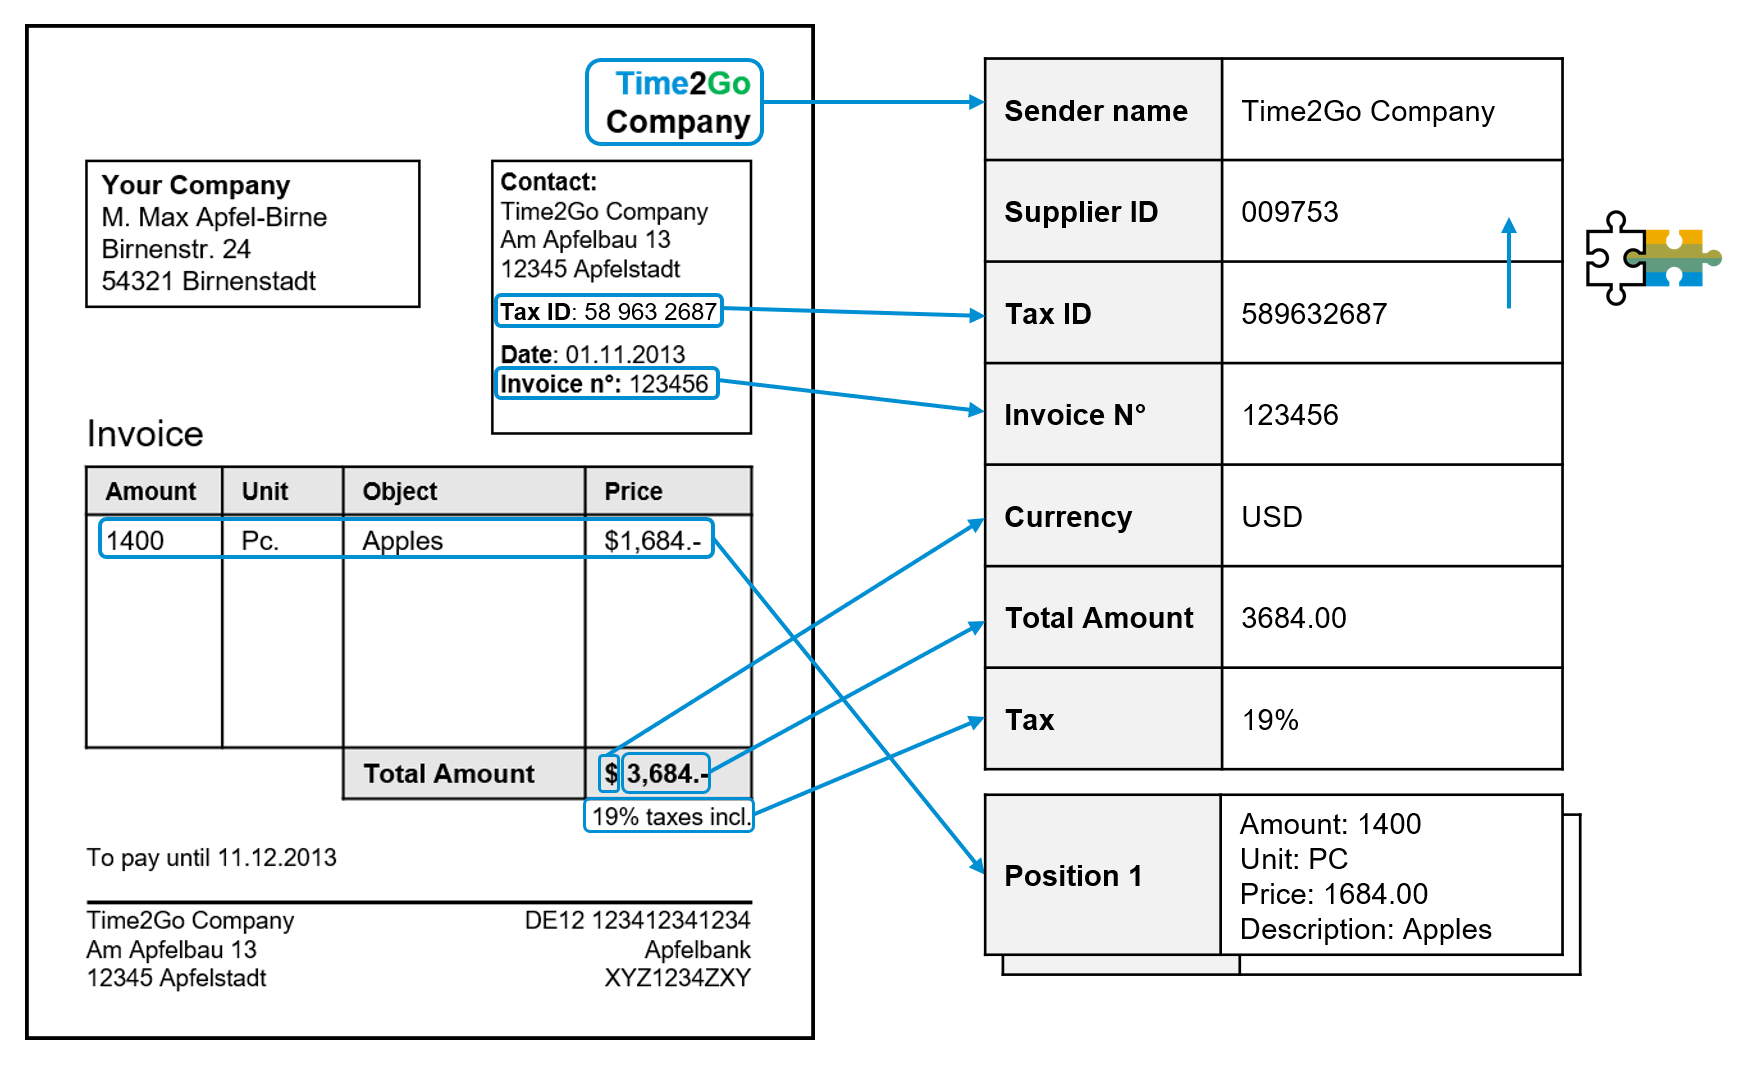
\includegraphics[width=1.0\linewidth]{./graphics/information_extraction.png}
  \captionof{figure}{Visuele representatie van information extraction}
\end{center}

\section{Conclusies}

Na het uitvoeren van dit onderzoek kan er geconcludeerd worden dat het zeker mogelijk is om met machine learning technologie bedrijfsdocument te analyseren en hieruit relevante masterdata te halen. Om een antwoord te geven op de onderzoeksvraag "Hoe kan machine learning-technologie worden toegepast om relevante masterdata uit bedrijfsdocumenten te halen?" is de proof of concept een voorbeeld van hoe dit gebruikt kan worden, doormiddel van de SAP Business Entity Recognition service.

Het antwoord op de deelvraag 'welke tools bestaan er om dergelijke oplossingen te maken' is terug te vinden in de literatuurstudie en toont aan dat er verschillende tools bestaan die gebruikt kunnen worden om dergelijke toepassingen te maken.
\section{Toekomstig onderzoek}

De resultaten van dit onderzoek kunnen gebruikt worden om een beeld te krijgen over hoe deze technologie precies werkt en toegepast kan worden. De proof of concept die gemaakt is kan verder uitgebreid worden om de resultaten te integreren in andere SAP applicaties, om ze zo verder te verwerken en te gebruiken. Verder kan het onderzoek ook dienen als basis naar andere machine learning methodes die gebruikt kunnen worden voor hetzelfde doel. 
\end{multicols}
\end{document}